% This is a template for the title page of any assignment or report.
% Owner: Bratin Mondal
% Usage:
% 1. Replace the placeholders with your information.
% 2. Add any additional information, if needed.
% 3. Add your university logo or any other image.
% 4. Add any other details, if needed, below the image.
% 5. Compile the document to see the output.

\documentclass[12pt]{article}
\usepackage{graphicx}
\usepackage{comment}
\usepackage{geometry}
\usepackage{hyperref}
\usepackage{float}
\renewcommand{\rmdefault}{ptm}
\newcommand{\bmr}[1]{\textcolor{red}{#1}}
\newcommand{\bmg}[1]{\textcolor{green}{#1}}
\newcommand{\bmb}[1]{\textcolor{blue}{#1}}
\newcommand{\bmp}[1]{\textcolor{magenta}{#1}}

% Define macros for information
\newcommand{\myName}{Bratin Mondal}
\newcommand{\myRollNumber}{21CS10016}
\newcommand{\myCourse}{CS60050 - Machine Learning}
\newcommand{\myAssignment}{2}
\newcommand{\myAssignmentTitle}{Song Popularity using Neural Networks}
\newcommand{\myUniversity}{Indian Institute of Technology Kharagpur}
\geometry{a4paper, margin=0.5in} % Adjust margins if necessary
\begin{document}
	
	\begin{titlepage}
		\centering
		
		{\Huge{\textbf{\myCourse}}}
		\vspace{0.5cm}
		
		{\Huge{Assignment \myAssignment}}
		
		\vspace{2cm}
		
		% Add your university logo or any other image here
		
\includegraphics[width=0.5\textwidth]{iit_kgp_logo.png}
		
		\vspace{2cm}
		
		% Add your report title here
		{\Huge\textbf{\myAssignmentTitle}}
		
		\vspace{2cm}
		
		% Add any other details like your name, date, etc.
		{\Large\textbf{\myName}} 
		\vspace{0.2cm}
		
		\large{\myRollNumber}    
		\vspace{2cm}
		
		% Add any additional information, if needed
		{\large\textit{Department of Computer Science and Engineering,}}
		
		{\large\textit{\myUniversity}}
		\vspace{0.3cm}
		
		% Two lines above the image
		\hrule 
		\vspace{0.5cm}
		
		% Add any other details, if needed, below the image
		
	\end{titlepage}
	
	\section{Problem Statement}
	
	\subsection{Objective:}
	This project aims to build neural network models for song popularity prediction based on a comprehensive set of music characteristics.
	
	\subsection{Model Specifications:} \label{subsec:model-specifications}
	\begin{enumerate}
		\item \textbf{ANN Specification 1}
		\begin{itemize}
			\item No of hidden layers: 1
			\item No. of neurons in hidden layer: 32
			\item Activation function in the hidden layer: Sigmoid
			\item 1 neuron in the output layer.
			\item Activation function in the output layer: Linear
			\item Optimization algorithm: Mini Batch Stochastic Gradient Descent (SGD)
			\item Loss function: Mean Squared Error (MSE)
			\item Learning rate: 0.01
			\item No. of epochs = 200
		\end{itemize}
		\item \textbf{ANN Specification 2}
		\begin{itemize}
			\item No of hidden layers: 2
			\item No. of neurons in the 1st hidden layer: 64
			\item No. of neurons in the 2nd hidden layer: 32
			\item Activation function in both the hidden layers: ReLU
			\item 1 neuron in the output layer.
			\item Activation function in the output layer: Linear
			\item Optimization algorithm: Mini Batch Stochastic Gradient Descent (SGD)
			\item Loss function: Mean Squared Error (MSE)
			\item Learning rate: 0.01
			\item No. of epochs = 200
		\end{itemize}
	\end{enumerate}
	
	\section{Modules}
	
	\subsection{Preprocess}
	\textbf{Purpose:} Preprocesses the input dataset by dropping duplicates, normalizing the data, and splitting it into training and testing datasets. 
	
	\subsection{DataLoader}
	\textbf{Purpose:} Loads the training and testing datasets and splits them into batches of size 32 for efficient training.
	
	\subsection{WeightInitialiser}
	\textbf{Purpose:} Initializes the weights of the dense layers in the neural network. It generates random weights within a specified range.
	
	\subsection{BiasInitialiser}
	\textbf{Purpose:} Initializes the biases of the dense layers in the neural network. It initializes biases for each layer to zero.
	
	\subsection{ForwardPass}
	\textbf{Purpose:} Performs the forward pass of the neural network. It calculates the outputs of each layer using the given input data and weights.
	
	\subsection{BackPropagation}
	\textbf{Purpose:} Performs the backward propagation of the neural network. It updates the weights and biases of the network based on the calculated gradients.
	
	\subsection{Training}
	\textbf{Purpose:} Trains the neural network by iterating over epochs. It utilizes forward pass and backpropagation to update model parameters and computes accuracy for each epoch.
	
	\subsection{Predict}
	\textbf{Purpose:} Predicts the labels for the training and testing datasets using the trained neural network model. It utilizes forward pass to obtain predictions.
	
	\begin{comment}
	\subsection{curAccu}
	\textbf{Purpose:} Calculates the accuracy of the model by comparing predicted labels with the ground truth labels.
	
	\subsection{BatchSplit}
	\textbf{Purpose:} Splits the dataset into batches of size 32 to facilitate mini-batch training.
	
	\subsection{gradSig}
	\textbf{Purpose:} Calculates the gradient of the sigmoid function. It's used in backpropagation for layers with sigmoid activation.
	
	\subsection{sig}
	\textbf{Purpose:} Calculates the sigmoid function. It's used as the activation function for the hidden layers.
	
	\subsection{reluDerivative}
	\textbf{Purpose:} Calculates the gradient of the ReLU function. It's used in backpropagation for layers with ReLU activation.
	
	\subsection{relu}
	\textbf{Purpose:} Calculates the ReLU function. It's used as the activation function for the hidden layers.
	\end{comment}


	\section{Helper Functions}
	\subsection{curAccu}
	\textbf{Purpose:} Calculates the accuracy of the model by comparing predicted labels with the ground truth labels.
	
	\subsection{BatchSplit}
	\textbf{Purpose:} Splits the dataset into batches of size 32 to facilitate mini-batch training.
	
	\subsection{gradSig}
	\textbf{Purpose:} Calculates the gradient of the sigmoid function. It's used in backpropagation for layers with sigmoid activation.
	
	\subsection{sig}
	\textbf{Purpose:} Calculates the sigmoid function. It's used as the activation function for the hidden layers.
	
	\subsection{reluDerivative}
	\textbf{Purpose:} Calculates the gradient of the ReLU function. It's used in backpropagation for layers with ReLU activation.
	
	\subsection{relu}
	\textbf{Purpose:} Calculates the ReLU function. It's used as the activation function for the hidden layers.
	

\section{Model} \label{sec:model}
\subsection{Data Preprocessing}
The input dataset is preprocessed by dropping duplicates and normalizing the data. 
\[
	A_{ij}^{\mathrm{processed}} = \frac{A_{ij} - \mu_j}{\sigma_j}	
\]
where $A_{ij}$ is the $j^{th}$ attribute of the $i^{th}$ data point, $\mu_j$ is the mean of the $j^{th}$ attribute, and $\sigma_j$ is the standard deviation of the $j^{th}$ attribute.
The dataset is then split into training and testing datasets in the ratio 80:20.
\subsection{Training}
The model specifications are same as described in \ref{subsec:model-specifications}. The target label is scaled using the MinMaxScaler using the fomula:
\[
    y^{\mathrm{processed}} = \frac{y}{100}
\]

The neural network is trained using the training dataset. The weights and biases are initialized using the WeightInitialiser and BiasInitialiser modules. The training is performed using the Mini Batch Stochastic Gradient Descent (SGD) optimization algorithm. The loss function used is Mean Squared Error (MSE). The learning rate is set to 0.01 and the number of epochs is set to 200. The model is trained using the forward pass and backpropagation modules. The accuracy of the model is calculated after 10 epochs and the training and testing accuracies are plotted against the number of epochs.
\subsection{Results}
The training and testing accuracies for the two models are plotted against the number of epochs. The training and testing accuracies for the two models are as follows:
\subsubsection{ANN Specification 1}
\begin{itemize}
	\item Training Accuracy: 1.901331769829969 \%
	\item Testing Accuracy: 2.1105527638190953 \%

\end{itemize}
\begin{figure}[H]
    \centering
    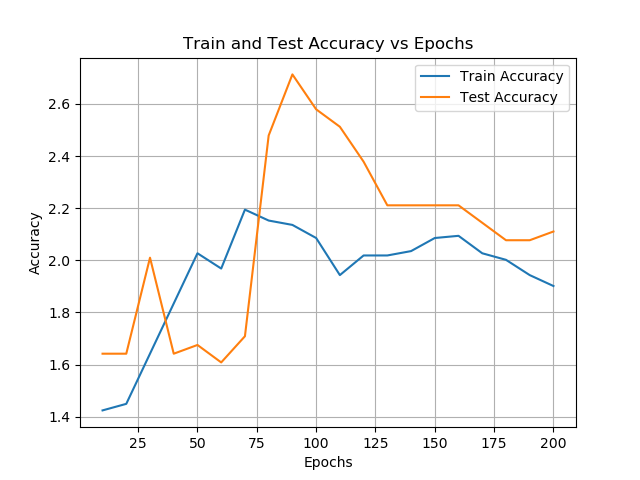
\includegraphics[width=0.55\textwidth]{Model_layer_32_1.png}
    \caption{Training and Testing Accuracies for ANN Specification 1}
    \label{fig:ann1}
\end{figure}
\subsubsection{ANN Specification 2}
\begin{itemize}
	\item Training Accuracy: 2.1105527638190953 \%
	\item Testing Accuracy: 2.1105527638190953 \%
\end{itemize}
\begin{figure}[H]
	\centering
	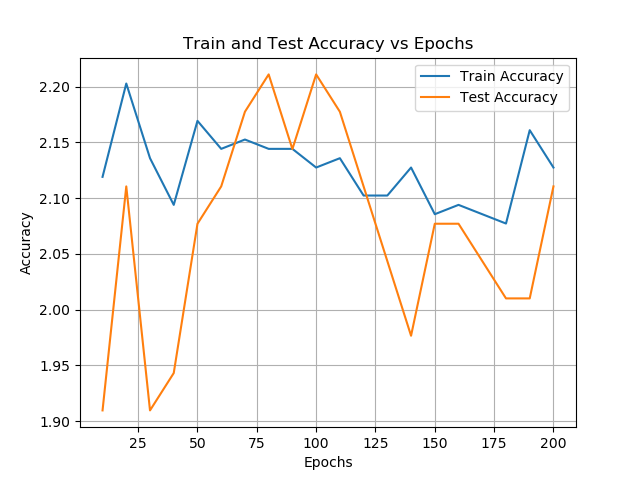
\includegraphics[width=0.55\textwidth]{Model_layer_64_32_1.png}
	\caption{Training and Testing Accuracies for ANN Specification 2}
	\label{fig:ann2}
\end{figure}

\section{Implementation using scikit-learn MLP} \label{sec:scikit-learn}
The same ANN specifications are implemented using the scikit-learn library. Two modeuls of the scikit-learn library are used: \textbf{MLPRegressor} and \textbf{MLR Classifier}.
\subsection{MLPClassifier}
\subsubsection{ANN Specification 1}
\begin{itemize}
	\item Training Accuracy: 4.640254627690761 \%
	\item Testing Accuracy: 2.4790619765494135 \%
\end{itemize}
\begin{figure}[H]
	\centering
	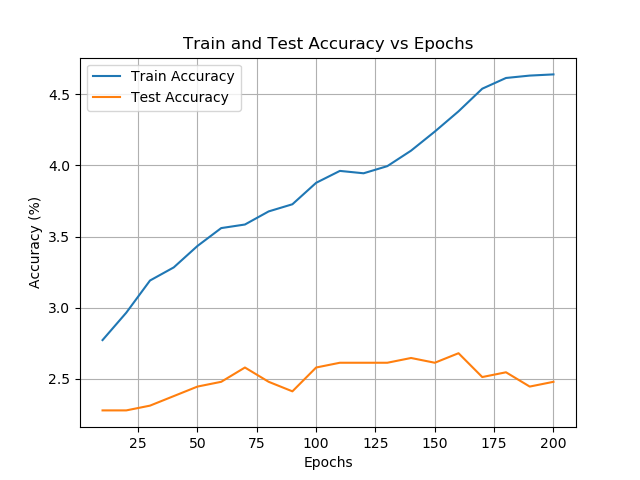
\includegraphics[width=0.55\textwidth]{scikit_learn_model_1_accuracy_comparison.png}
	\caption{Training and Testing Accuracies for MLPClassifier Specification 1}
	\label{fig:mlp1}
\end{figure}
\subsubsection{ANN Specification 2}
\begin{itemize}
	\item Training Accuracy: 8.468045899991624 \%
	\item Testing Accuracy: 1.2730318257956448 \%
\end{itemize}
\begin{figure}[H]
	\centering
	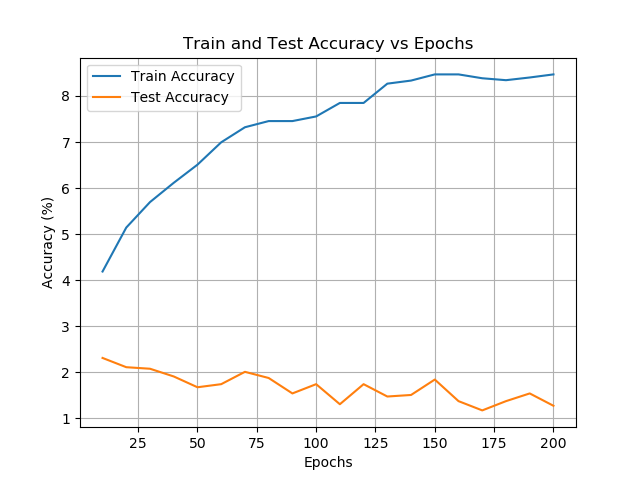
\includegraphics[width=0.55\textwidth]{scikit_learn_model_2_accuracy_comparison.png}
	\caption{Training and Testing Accuracies for MLPClassifier Specification 2}
	\label{fig:mlp2}
\end{figure}
\subsection{MLPRegressor}
\subsubsection{ANN Specification 1}
\begin{itemize}
	\item Training Accuracy: 1.6249267107797973 \%
	\item Testing Accuracy: 2.0435510887772192 \%
\end{itemize}
\begin{figure}[H]
	\centering
	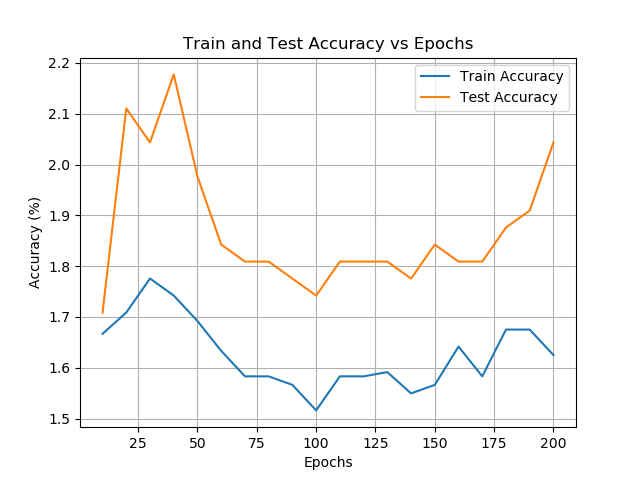
\includegraphics[width=0.55\textwidth]{scikit_learn_model_3_accuracy_comparison.png}
	\caption{Training and Testing Accuracies for MLPRegressor Specification 1}
	\label{fig:mlpr1}
\end{figure}
\subsubsection{ANN Specification 2}
\begin{itemize}
	\item Training Accuracy: 1.7840690175056537 \%
	\item Testing Accuracy: 1.574539363484087 \%
\end{itemize}
\begin{figure}[H]
	\centering
	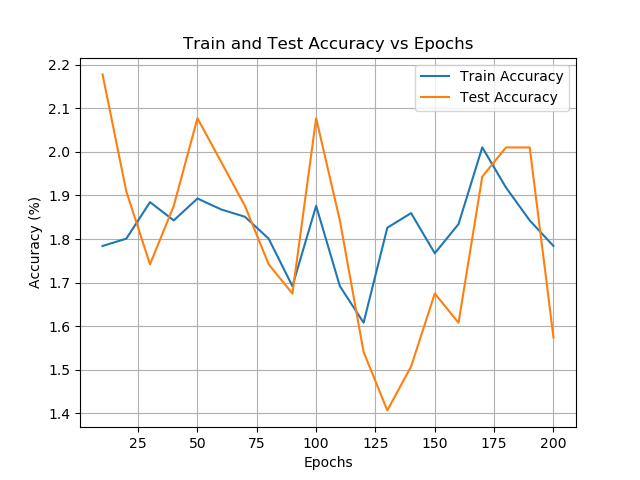
\includegraphics[width=0.55\textwidth]{scikit_learn_model_4_accuracy_comparison.png}
	\caption{Training and Testing Accuracies for MLPRegressor Specification 2}
	\label{fig:mlpr2}
\end{figure}
\section{Improving the Model} \label{sec:improving-model}
Using the scikit-learn library, we observed that MLPClassifier performs better than MLPRegressor on training set. We further use this idea to improve our model. Instead of predicting the popularity as a target, we create 101 classes for the popularity and use softmax activation function in the output layer and cross entropy loss function and choose the class with the highest probability as the predicted popularity. We use the same ANN specifications as described in \ref{subsec:model-specifications} along with some minor changes.
\begin{enumerate}
	\item \textbf{ANN Specification 1}
	\begin{itemize}
		\item No of hidden layers: 1
		\item No. of neurons in hidden layer: 32
		\item Activation function in the hidden layer: Sigmoid
		\item 101 neurons in the output layer.
		\item Activation function in the output layer: Softmax
		\item Optimization algorithm: Mini Batch Stochastic Gradient Descent (SGD)
		\item Loss function: Categorical Cross Entropy
		\item Learning rate: 0.01
		\item No. of epochs = 200
	\end{itemize}
	\item \textbf{ANN Specification 2}
	\begin{itemize}
		\item No of hidden layers: 2
		\item No. of neurons in the 1st hidden layer: 64
		\item No. of neurons in the 2nd hidden layer: 32
		\item Activation function in both the hidden layers: ReLU
		\item 101 neurons in the output layer.
		\item Activation function in the output layer: Softmax
		\item Optimization algorithm: Mini Batch Stochastic Gradient Descent (SGD)
		\item Loss function: Categorical Cross Entropy
		\item Learning rate: 0.01
		\item No. of epochs = 200
	\end{itemize}
\subsection{Results}
The training and testing accuracies for the two models are plotted against the number of epochs. The training and testing accuracies for the two models are as follows:
\subsubsection{ANN Specification 1}
\begin{itemize}
	\item Training Accuracy: 3.769159896138705 \%
	\item Testing Accuracy: 2.3450586264656614 \%
\end{itemize}
\begin{figure}[H]
	\centering
	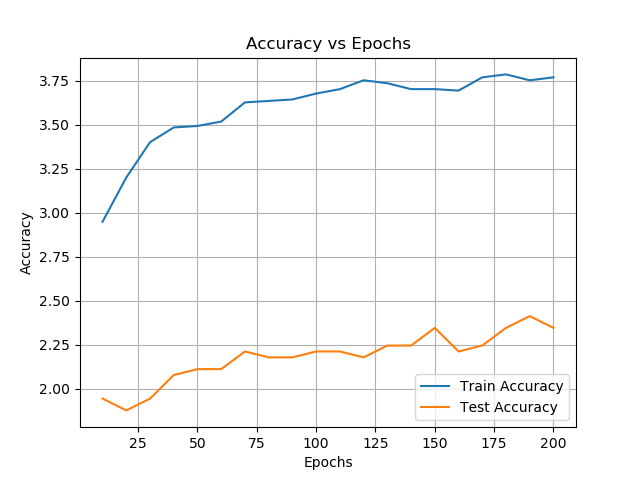
\includegraphics[width=0.55\textwidth]{Model_improved_layer_32_101.png}
	\caption{Training and Testing Accuracies for ANN Specification 1}
	\label{fig:ann1}
\end{figure}
\subsubsection{ANN Specification 2}
\begin{itemize}
	\item Training Accuracy: 3.149342490995896 \%
	\item Testing Accuracy: 2.4120603015075375 \%
\end{itemize}
\begin{figure}[H]
	\centering
	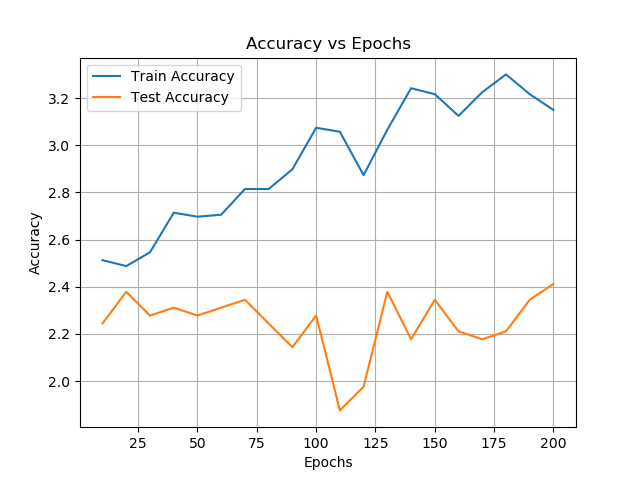
\includegraphics[width=0.55\textwidth]{Model_improved_layer_64_32_101.png}
	\caption{Training and Testing Accuracies for ANN Specification 2}
	\label{fig:ann2}
\end{figure}
\section{Conclusion}
We observe that the improved model performs better than the previous models. The training and testing accuracies are higher than the previous models. The improved model is able to predict the popularity of the songs with higher accuracy. We also note that since there are very less number of attributes, the model structure is not very complex and the target variable ranges over a large range of \(1-100\), the model specifications could not acheive very high accuracy. We can further improve the model by adding more attributes, increasing the complexity of the model and changes in the loss function and activation functions.
\appendix
\section{Appendix}
\subsection{Running the Code}
Use the makefile to run the code. \\
For \autoref{sec:model} enter the following command:
\begin{verbatim}
	make model
\end{verbatim}
For \autoref{sec:scikit-learn} enter the following command:
\begin{verbatim}
	make test_scikit_learn 
\end{verbatim}
For \autoref{sec:improving-model} enter the following command:
\begin{verbatim}
	make mymodel
\end{verbatim}
See \textit{readme.md} for more details.
\end{document}